%%%%%%%%%%%%%%%%%%%%%%%%%%%%%%%%%%%%%%%%%%%%%%%%%%%%%%%%%%%%%%%%%%%%%%
%%%%%%%%%%%%%%%%%%%%%%%%%%%%%%%%%%%%%%%%%%%%%%%%%%%%%%%%%%%%%%%%%%%%%%
\chapter{Boundary conditions}



%%%%%%%%%%%%%%%%%%%%%%%%%%%%%%%%%%%%%%%%%%%%%%%%%%%%%%%%%%%%%%%%%%%%%%
\section{Implementation of periodic boundary conditions}

The periodic boundary conditions which are implemented are suitable only for
rectangular boxes with surfaces oriented parallel to the coordinate planes.

Each pair of boundary conditions defines master and corresponding slave
nodes. The slave nodes get a pointer to the degrees of freedom of their
masternode. This means, that the size of the dofset is reduced in comparison
to a calculation without periodic boundary nodes!

In addition to that, master and slave nodes have to be owned by the same proc
and are only allowed to be ghosted in pairs to be able to assign the degrees
of freedom.

%%%%%%%%%%%%%%%%%%%%%%%%%%%%%%%%%%%%%%%%%%%%%%%%%%%%%%%%%%%%%%%%%%%%%%
\subsubsection{Construction of the master slave matching}
The master slave matching is constructed using a parallel octree search. For
this purpose, we search for each master node the closest slave node on all
processors. For this purpose, one of the slaves coordinates is modified
in such a way that the new coordinate is in the master plane.

%%%%%%%%%%%%%%%%%%%%%%%%%%%%%%%%%%%%%%%%%%%%%%%%%%%%%%%%%%%%%%%%%%%%%%
\subsubsection{Redistribution of nodes}
The nodes are redistributed among the processors. Each couple is owned by a
unique processor and if a slave is ghosted on a processor, the corresponding
master is ghosted there, too.

%%%%%%%%%%%%%%%%%%%%%%%%%%%%%%%%%%%%%%%%%%%%%%%%%%%%%%%%%%%%%%%%%%%%%%
\subsubsection{Renumbering the degrees of freedom}
All slave nodes do not get their own degrees of freedom. Instead, their index
for the access of the degrees of freedom from nodes is set to the index of
their corresponding masternode. (This is what makes it necessary to ghost the
master if you ghost the slave)

%%%%%%%%%%%%%%%%%%%%%%%%%%%%%%%%%%%%%%%%%%%%%%%%%%%%%%%%%%%%%%%%%%%%%%
\subsubsection{Periodic boundary conditions and IO}
The assignement of periodic boundary conditions changes the numbering of the
degrees of freedom. For this reason, the conditions have to be written to the
output to be able to reconstruct the dof pattern during the setup of the
discretisation in the postprocessing filters.

%%%%%%%%%%%%%%%%%%%%%%%%%%%%%%%%%%%%%%%%%%%%%%%%%%%%%%%%%%%%%%%%%%%%%%
\subsubsection{Periodic boundary combined with additional 
  (Dirichlet) conditions}
For periodic boundary conditions several nodes correspond to the same set of
degrees of freedom. If you want to assign an additional condition to such a
node make sure that you assign the same condition to all corresponding nodes.

This necessity is caused by the hirarchical way in which conditions are
assigned to the dofs. Each node belonging to this condition sets its condition
onto the degrees of freedom, overriding previously set conditions.
So, if you want to make sure that this condition is set, you have to assign it
to all coressponding nodes or the result depends on the order in which the
nodes in the condition are processed.

Another thing of practical interest might be that the assignement of periodic
boundary conditions may lead to purely Dirichlet constrained problems
(examples channel flow or a Couette flow). 

%%%%%%%%%%%%%%%%%%%%%%%%%%%%%%%%%%%%%%%%%%%%%%%%%%%%%%%%%%%%%%%%%%%%%%
\section{Implemented boundary conditions}

%%%%%%%%%%%%%%%%%%%%%%%%%%%%%%%%%%%%%%%%%%%%%%%%%%%%%%%%%%%%%%%%%%%%%%
\subsection{Lung related boundary conditions}

%%%%%%%%%%%%%%%%%%%%%%%%%%%%%%%%%%%%%%%%%%%%%%%%%%%%%%%%%%%%%%%%%%%%%%
\subsubsection*{Sinus Curve for Alveolar Pressure as Boundary Condition}

The lung load curve is a sinus curve (actually implemented is 1-cos),
which oscillates between the Ppeep and 1. In order to avoid to much
shock to the structure the curve has a sin curve as starting curve.
In case Phase = 0, Phase is set to the value $1/Freq$ \bigskip
\par For $T<Phase$ the function is described by 
\begin{center}
$0.5*Ppeep*(1 - cos(\frac{\pi*t}{Phase}))$
\end{center}
\par else it is described by 
\begin{center}
$0.5*(1-Ppeep)*(1 - cos(2*\pi*Frequ*(t - Phase))) + Ppeep$
\end{center}

\begin{center}
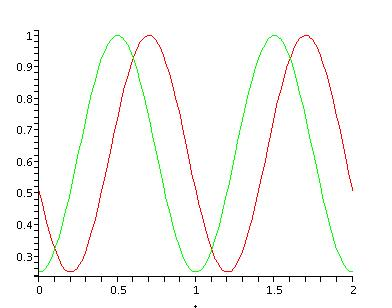
\includegraphics[width=70mm]{figures/phase}
\end{center}

\begin{center}
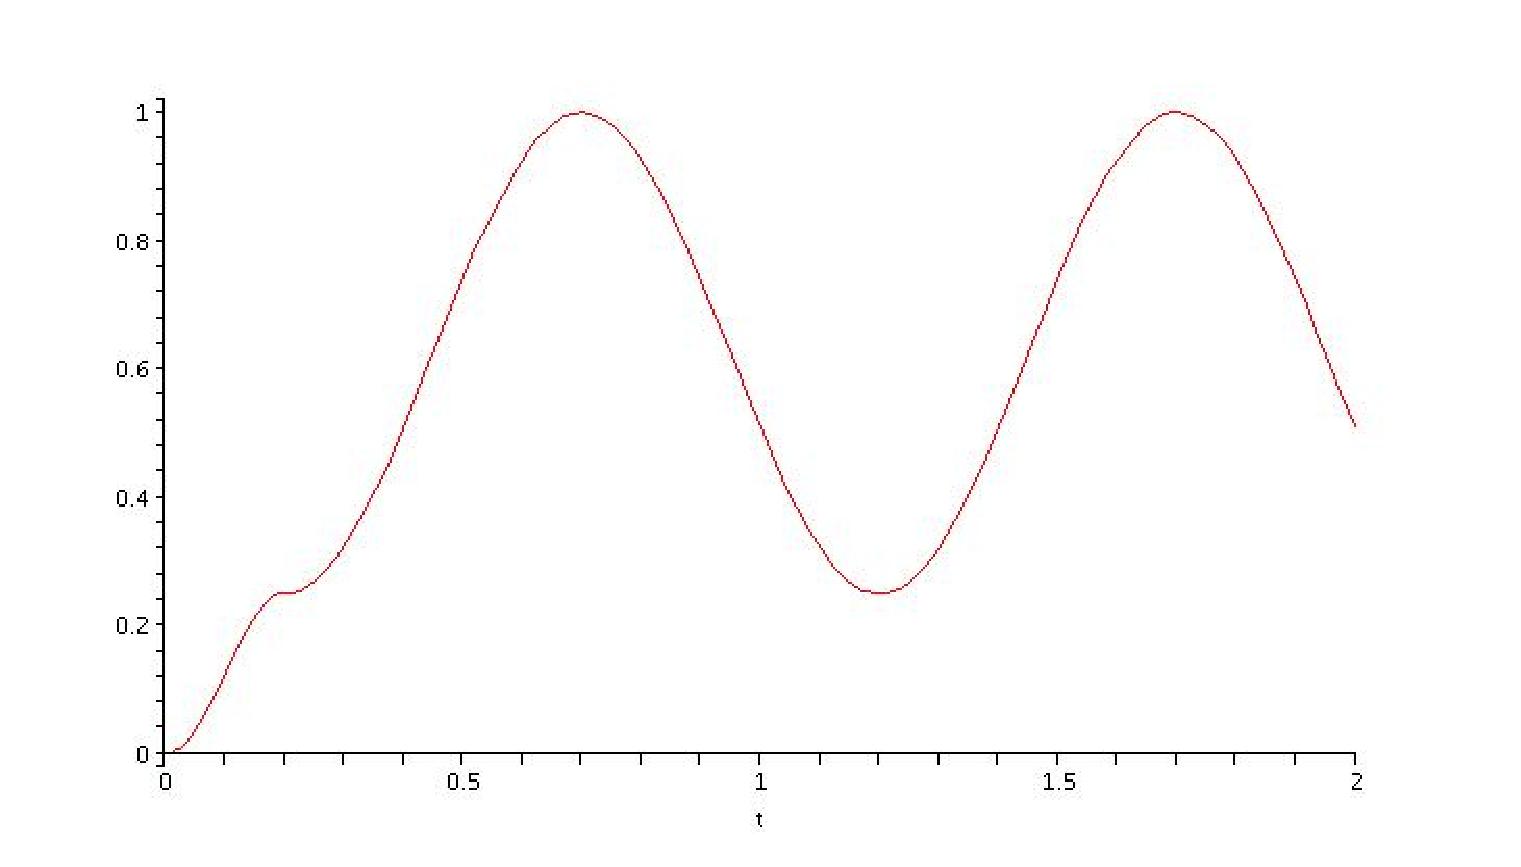
\includegraphics[width=70mm]{figures/start}
\end{center}


\paragraph*{Parameters to describe the curve:\\}

\begin{tabular}{|c|c|p{125mm}|}
	\hline
	c1	& Frequ	& Frequency of the oscillation (in case time is in s, then Freq is in Hz) \\
	\hline
	c2	& pPEEP 	& Percentual peep (ration of peep to maximum pressure)\\
	\hline
	c3	& Phase 	& Phase\\
	\hline
\end{tabular}

\paragraph*{Line to describe the curve in the input file:\\}
{\tt CURVE1 on LungSinus FUNC Frequ 1.0 pPEEP 0.2 Phase 0.0}


\paragraph*{Modified files:\\}

\begin{itemize}
	\item {\tt src/global\_full/global\_timecurve.c}
	\par \noindent lung curve implemented as curve -10 of explicit curves

	\item {\tt src/input\_full/input\_curves.c}
	\par \noindent redirected Lung Function to explicit framework

	\item {\tt src/headers/curve.h}
	\par \noindent added c3
\end{itemize}


%%%%%%%%%%%%%%%%%%%%%%%%%%%%%%%%%%%%%%%%%%%%%%%%%%%%%%%%%%%%%%%%%%%%%%
\subsubsection*{Curve for Alveolar Pressure as Boundary Condition}

The function describes the alveolar pressure during mechanical ventilation.
Its based on the data of Claudius Stahl, University of Freiburg.
It oscillates beetweeen the percentual peep an the value 1.
One respiration cycle is composed of the inspiration, the end-inspiratory plateau and the expiration.

\begin{itemize}
	\item The inspiration is described by a linear rise starting with the pressure of the percentual peep and ending at the time $t_{insp}$ with the pressure 1.
	\item The end-inspiratory plateau is described by an exponential decrease \linebreak $A*exp(-B*T)+C$ sarting at time $t_{insp}$ with the pressure 1. The shape of the function can be defined by the parameters B and C.
	\item The expiration is described by an exponential decrease $a*exp(-b*T)+c$. It starts at the end of the end-inspiratory plateau and ends at the time $t_{insp}+t_{plateau}+t_{exp}$ with the pressure of the percentual peep. The shape of the function can be defined by the parameter b.
	\item In order to avoid to much shock to the structure the curve has a starting phase before the first respiration cycle. It is described by a quadratic function, whitch starts at time zero with value and gradient zero and ends at the beginning of the inspiration with the same value and gradient as the inspiration.
\end{itemize}
\bigskip \par


\begin{center}
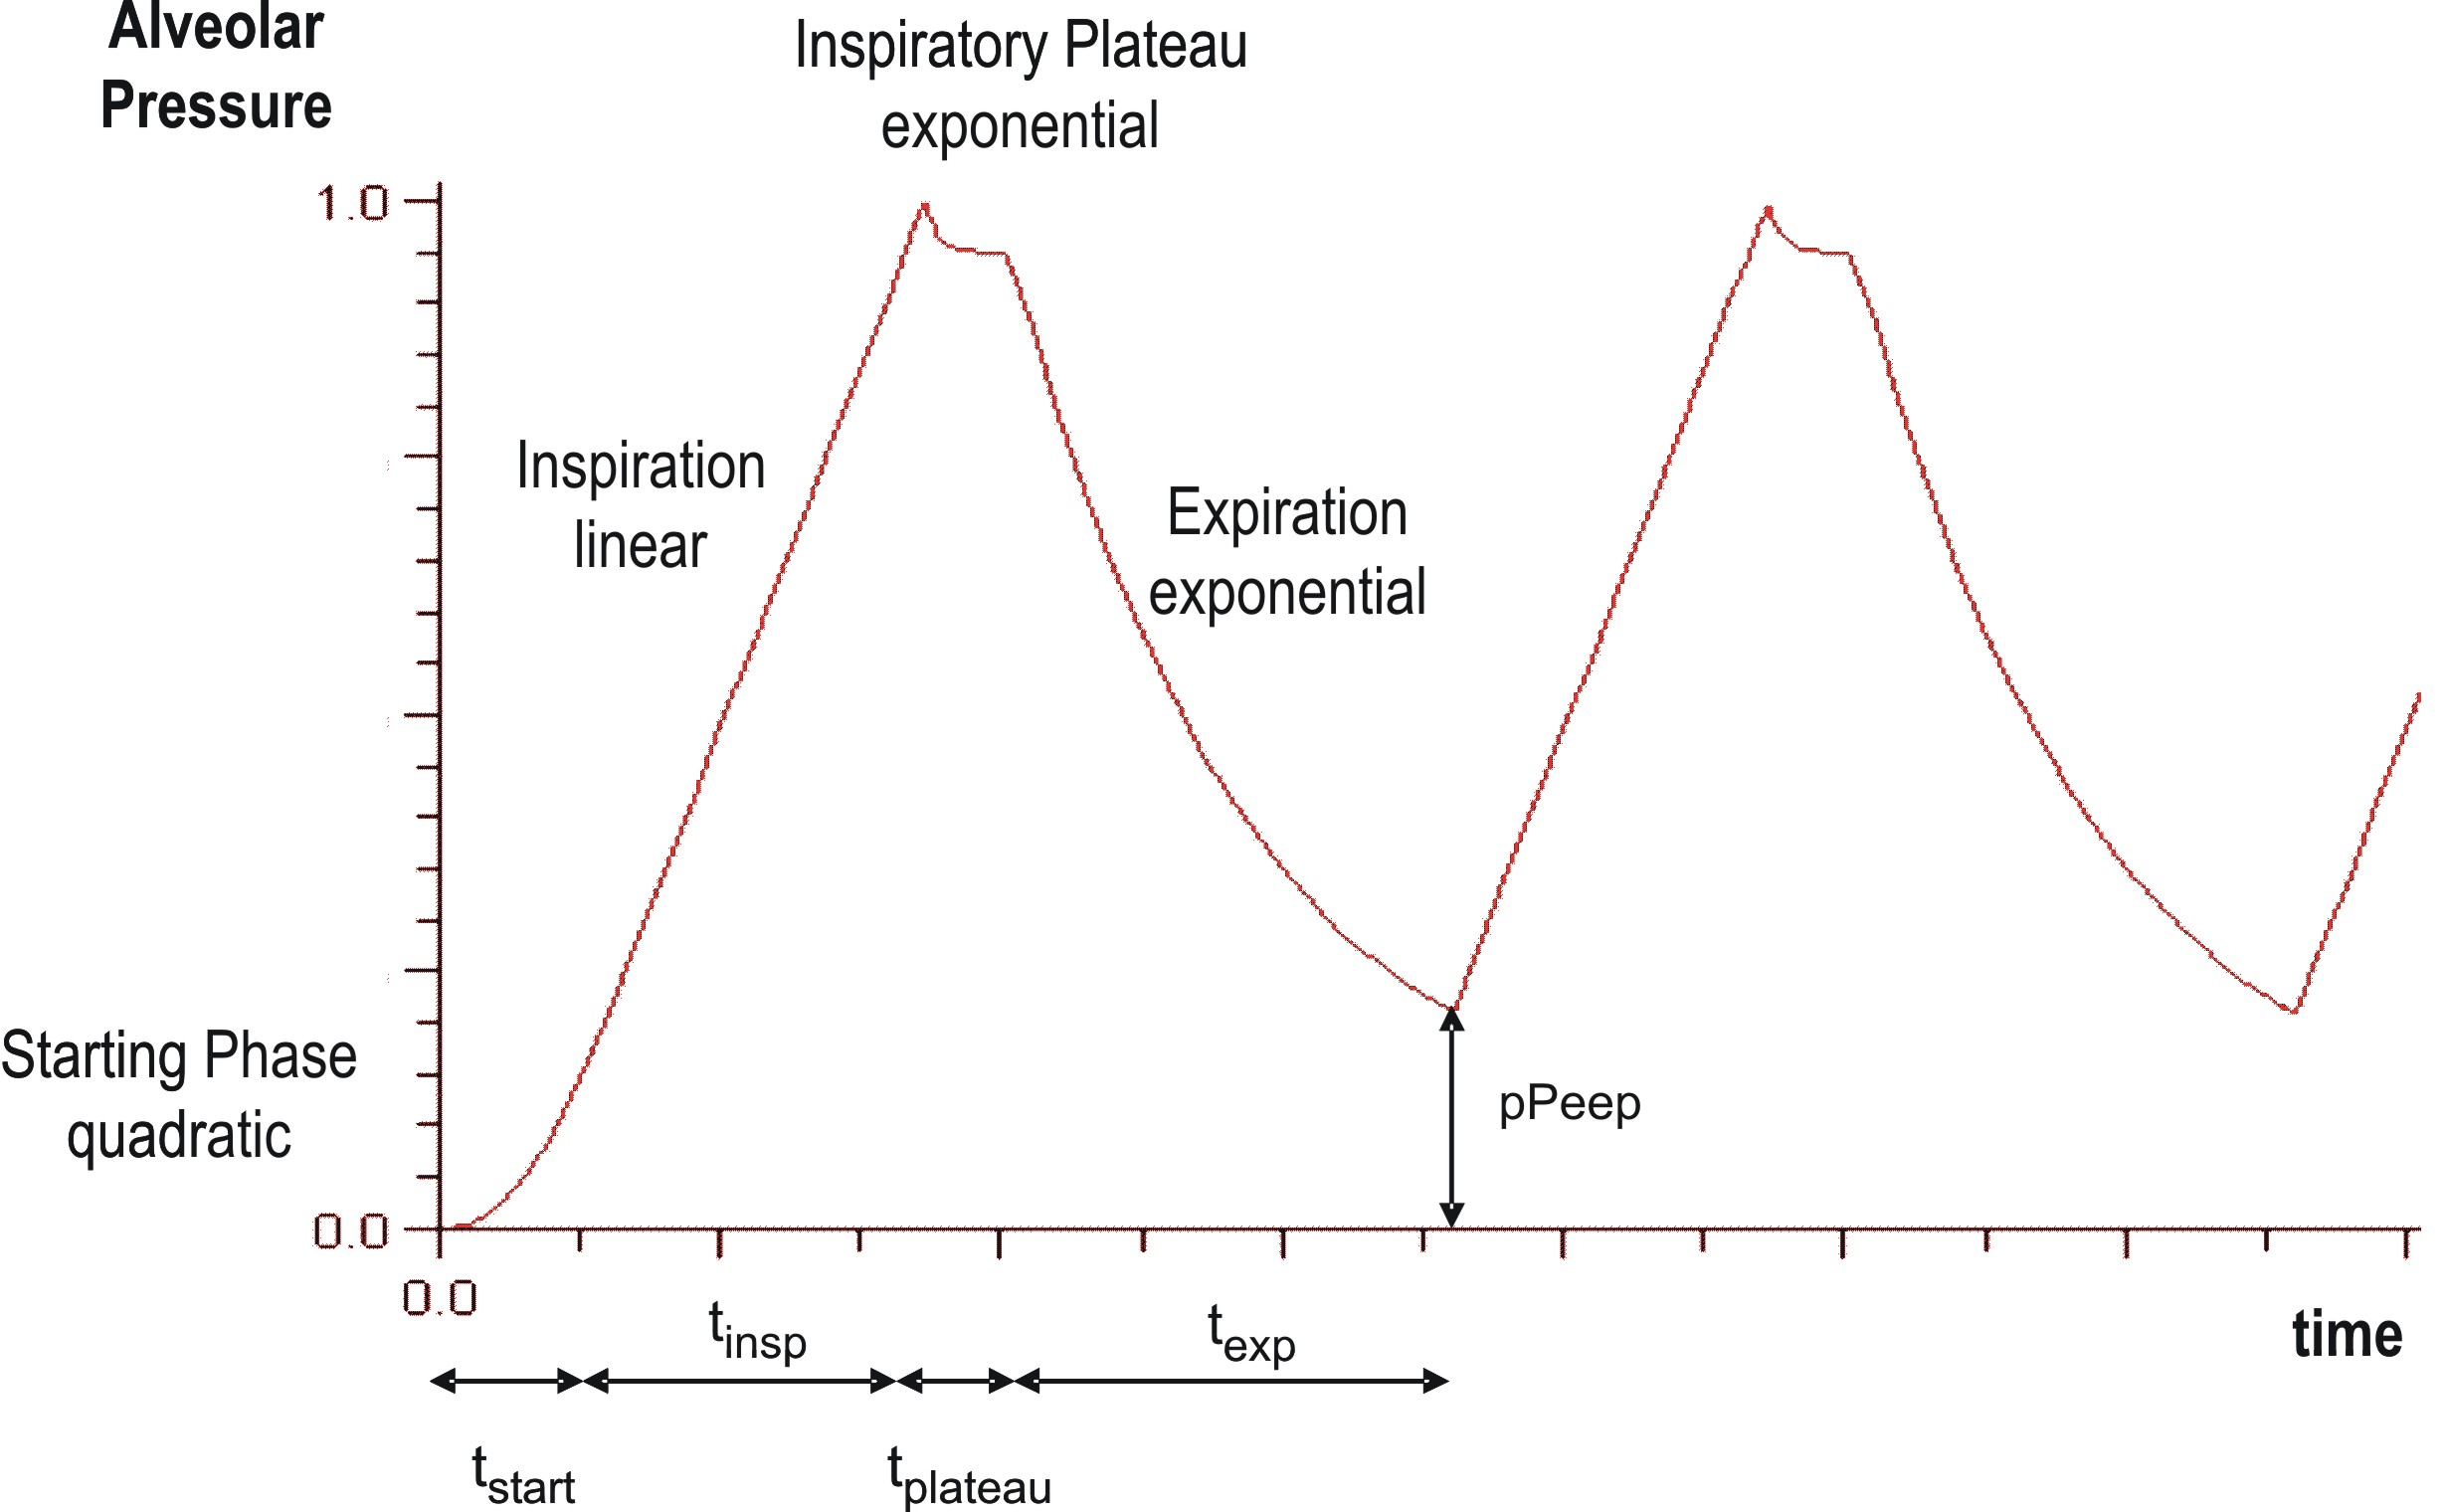
\includegraphics[width=100mm]{figures/PAlveolar}
\end{center}

\paragraph*{Parameters to describe the curve:\\}

\begin{tabular}{|c|c|p{125mm}|}
	\hline
	c1	& Frequ	& Frequency of the oscillation (in case time is in s, then Freq is in Hz) \\
	\hline
	c2	& pPEEP 	& Percentual peep (ration of peep to maximum pressure)\\
	\hline
	c3	& I/E 	& Ratio of inspiration time (including the end-inspiratory plateau) to expiration time \\
	\hline
	c4	& IPause/I 	& Ratio of period of the end-inspiratory plateau to complete inspiration time (including the end-inspiratory plateau)\\
	\hline
	c5	& ShapeIPauseB & Parameter to describe the exponential function for the end-inspiratory plateau (must be $>0$)\\
	\hline
	c6	& ShapeIPauseC & Parameter to describe the exponential function for the end-inspiratory plateau (must be beetween the percentual peep and the value 1)\\
	\hline
	c7	& ShapeEB 	& Parameter to describe the exponential function for the expiration (must be $>0$)\\
	\hline
\end{tabular}

\bigskip \par \noindent The periods $t_{insp}$, $t_{plateau}$ and $t_{exp}$ are calculated by the parameters c1, c3 and c4.

\paragraph*{Line to describe the curve in the input file:\\}
{\tt CURVE1 on LungReal FUNC Frequ 0.5 pPEEP 0.2 I/E 0.9 IPause/I 0.2 ShapeIPauseB 24.8 \\ ShapeIPauseC 0.94 ShapeEB 1.5}

\subsection*{Modified files}
\begin{itemize}
	\item {\tt src/global\_full/global\_timecurve.c}
	\par \noindent lung curve implemented as curve -12 of explicit curves

	\item {\tt src/input\_full/input\_curves.c}
	\par \noindent redirected Lung Function to explicit framework

	\item {\tt src/headers/curve.h}
	\par \noindent added c4, c5, c6, and c7
\end{itemize}
